\documentclass{beamer}

\usepackage{main}

\begin{document}

\begin{frame}[noframenumbering]
    \begin{center}
    
        \begin{columns}
            \column{.4\textwidth}
    
            
\includegraphics[width=0.4\textwidth, right]{images/acs.jpg}
    
    		\column{.6\textwidth}
    
            {
                \tiny
    
                \textbf{\detailcountry} \\
                \textbf{\detailuniversity} \\
                \textbf{\detailfaculty} \\
                \textbf{\detailspecialization} \\
            }
        \end{columns}
    
        \vspace*{1.5cm}
    
        \textbf{\huge{\detailtitle}}
    
        \vspace*{1cm}

        \tiny
        \begin{tabular*}{\textwidth}{l@{\extracolsep{\fill}}r}
            \textbf{Supervisor} & \textbf{Students}\\
            \tiny \detailadviser & \tiny \detailfirstauthor\\
             & \tiny \detailsecondauthor
        \end{tabular*}

        \vspace*{1.5cm}

        \textbf{\detailcity} \\
        \textbf{\detaildate}

    \end{center}
\end{frame}

\begin{frame}{Context} \pause
	\begin{itemize}
		\item Widespread use of executables \pause
	    \item Increase of vulnerabilities \pause
	    \item Approaches \pause
		    \begin{itemize}
		        \item Manual \pause
		        \item Automated
	        \end{itemize}
	\end{itemize}
\end{frame}

\begin{frame}{Cyber Reasoning Systems} \pause
	\begin{itemize}
		\item Automated vulnerability detection, exploitation and patching \pause
	    \item Developed solutions \pause
	    \begin{itemize}
    	    \item DARPA's Cyber Grand Challenge \pause
    		    \begin{itemize}
    		        \item Mayhem \pause
    	        \end{itemize}
            \item HaCRS
        \end{itemize}
	\end{itemize}
\end{frame}

\begin{frame}{Motivation} \pause
	\begin{itemize}
		\item Not applicable on common operating systems\pause
	    \item No longer maintained \pause
	    \item Commercial \pause
	\end{itemize}
\end{frame}

\begin{frame}{Objectives} \pause
	\begin{itemize}
		\item Study of the proposed CRSs \pause
	    \item Creation of a functional and open-source prototype \pause
	    \item Initial limitation for x86 ELF executables \pause
	\end{itemize}
\end{frame}

\begin{frame}{Bird's Eye View Architecture} \pause
	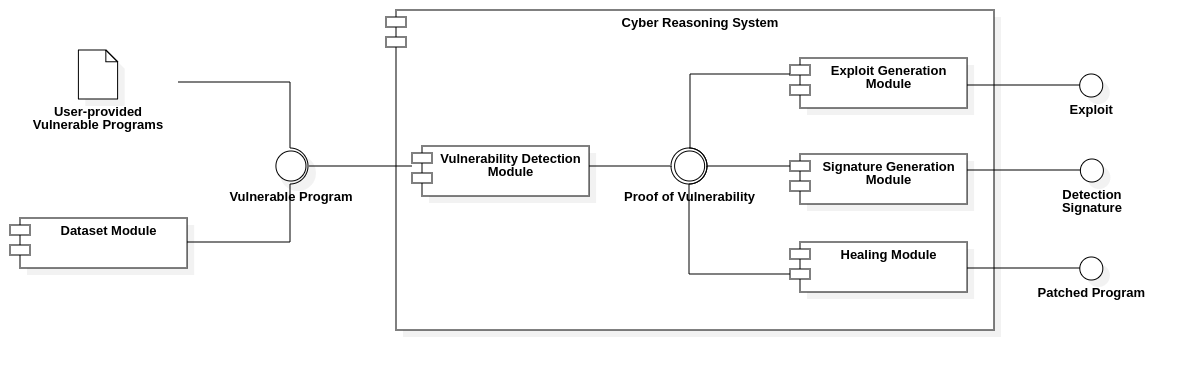
\includegraphics[width=\textwidth, center]{images/architecture.png}
    \captionsetup{justification=centering,margin=1cm}
\end{frame}

\begin{frame}{Current Status} \pause
	\begin{itemize}
		\item Researching the field of CRS \pause
	    \item Proposal of an architecture \pause
	    \item Started implementation in Python 3 \pause
		    \begin{itemize}
		        \item Dataset \pause
		        \item Attack surface approximation
	        \end{itemize}
	\end{itemize}
\end{frame}

\begin{frame}{Further Development} \pause
	\begin{itemize}
		\item SotA for the proposed technologies \pause
	    \item Completion of the vulnerability detection module
	\end{itemize}
\end{frame}

\begin{frame}{Conclusions} \pause
	\begin{itemize}
		\item Automated approach for binary analysis \pause
	    \item Novelty of CRS \pause \textit{(but with the presented downsides)} \pause
	    \item Proposed CRS study and prototype
	\end{itemize}
\end{frame}

\end{document}